\chapter{引论}
\section{系统和网}
\textbf{通信系统}是将用户(信源)要求传递的信息转移到另一个用户(信宿)的全部软硬通信设备。\\
通信过程:信源-发送器-信道-接收器-信宿\\
一条线路:连接两个话机的这一对线。
\subsection{连接方式}
\begin{description}
	\item[全联结网] $ C^2_n = \frac{n(n-1)}{2} $
	\item[采用中央 交换的方式] $ C^2_n -- n $,当任意两个用户要通话时,
	由交换机将它们连通,通
	话完毕将线路拆除,供其
	他用户使用
\end{description}
网络的结构的变化:点-点,全联通,交换式\\
建立大规模通信网需要引入层次交换。
\begin{figure}
	\centering
	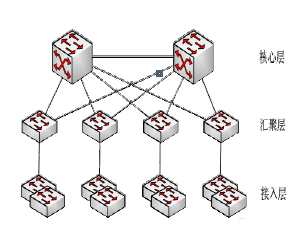
\includegraphics[width=0.7\linewidth]{figures/screenshot019}
	\caption{}
	\label{fig:screenshot019}
\end{figure}
终端设备-传输设备-交换设备-传输设备-终端设备\\
\textbf{交换:}
\begin{description}
	\item[思想] 动态按需分配
	\item[目的] 网络资源共享,降低通信成本
\end{description}
用户到交换机通过\textbf{用户线}连接,交换机之间通过\textbf{中继线}连接。
\subsection{等级制网络结构}
全部节点分成多个等级,每个节点属于某
个等级,低等级节点与管辖它的高等级节点相连,形成多级
汇接辐射结构。
\begin{enumerate}
	\item 高等级通信繁忙时,可连接成\textbf{网状结构}
	\item 某些节点间的联系十分密切,则可以建立直接连接。
\end{enumerate}
\subsubsection{电话网}
电话网络结构的演变:减少等级->无级动态网,现在的长途电话网结构为\textbf{二级}\\
传统电话网分为:
\begin{description}
	\item[本地网] 在\textbf{同一编号区域}范围内,由若干端局,或者由若干端局与汇接局及局间中继线、用户线和话机终端等组成的电话网
	\item[长途网] 指在全国范围内,由端局、汇接局和若干个长途局组成。
\end{description}
\begin{figure}[H]
	\centering
	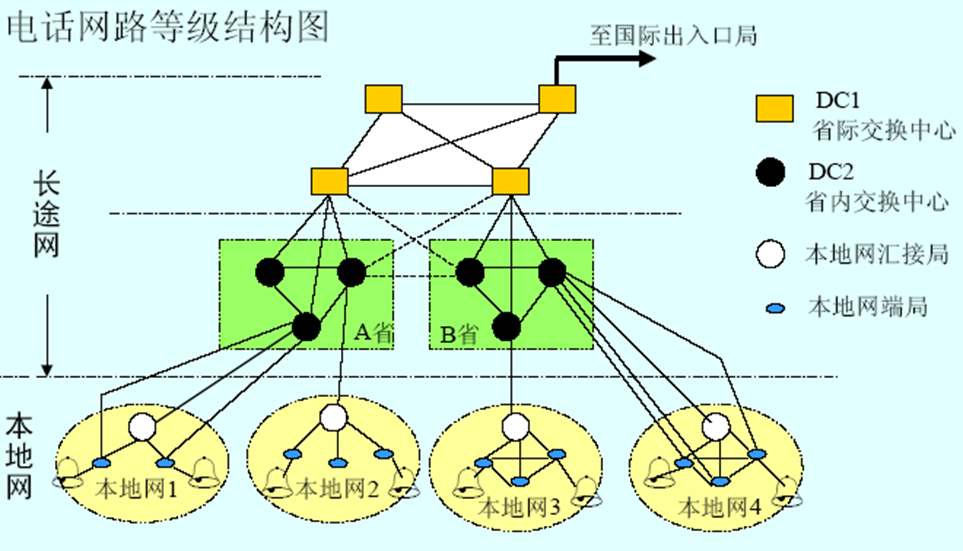
\includegraphics[width=0.7\linewidth]{figures/screenshot020}
	\caption{}
	\label{fig:screenshot020}
\end{figure}
\begin{description}
	\item[DC1] 省际交换中心,汇接所在省的省际长途来话、去话话务,以及所在本地网的长途终端话务
	\item[省内] 汇接所在本地网的长途终端话务
\end{description}
\subsubsection{因特网}
多级结构的因特网,主机到主机的通信可能经过多种 ISP。\\
下一代网络的系统结构:
接入层,传送层,控制器,业务/应用层。 四层。
\section{通信网的类型}
按不同方式有不同分类,如按距离分,按业务分。
\section{通信网的组成要素}
通信网是通信系统的系统。
通信网的“硬件":完成\textbf{接入、传输和交换}
\begin{enumerate}
	\item 终端机,信息的产生者和使用者
	\item 传输线路,UTP非屏蔽双绞线
	,STP屏蔽双绞线...,有线传输、无线传输。传输线路复用。
	\item 交换设备和业务节点\\
	交换方式
	\begin{enumerate}
		\item 电路交换,以电路联接为目的的交换方式是电路交换方式。\textbf{面向连接}。\\
		分为三个阶段:\textbf{建立连接、通信、释放连接}。\\
		特点:
		\begin{enumerate}
			\item 局内用户间连通,用户-用户。
			\begin{figure}[H]
				\centering
				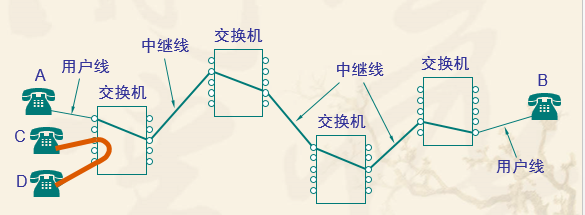
\includegraphics[width=0.7\linewidth]{figures/screenshot021}
				\caption{}
				\label{fig:screenshot021}
			\end{figure}
			\item 本局用户与有中继线联结的用户接通(用户—中继线—用户 )
			\begin{figure}[H]
				\centering
				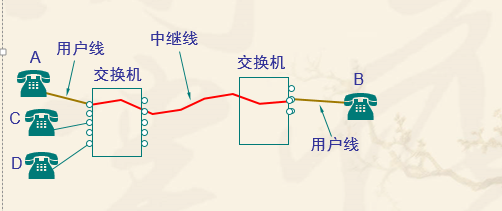
\includegraphics[width=0.7\linewidth]{figures/screenshot022}
				\caption{}
				\label{fig:screenshot022}
			\end{figure}
			\item 纯交换,中继线与中继线
			\begin{figure}[H]
				\centering
				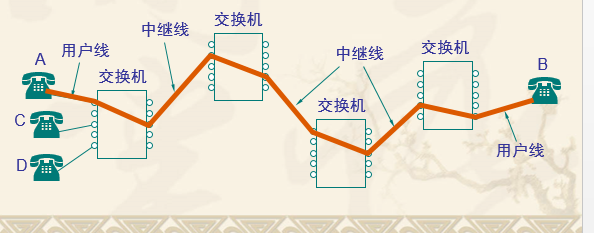
\includegraphics[width=0.7\linewidth]{figures/screenshot023}
				\caption{}
				\label{fig:screenshot023}
			\end{figure}
		\end{enumerate}
		缺点:网络资源(包括线路和交换设备)的利用不充分。
		\item 报文交换,将整个报文作为一个整体进行\textbf{存储-转发}
		\item 分组交换,把一份报文分解成若干段,每一段组装成为一个分组(Packet),交换机以分组作为存储、处理和传输单元。\\
		\textbf{转发原理}:将需要传输的数据组装成分组,标上地址信息发往网络,\textbf{网络各结点根据分组的地址},一级级地转发到目的地。
		分组交换的两种形式:
		\begin{description}
			\item[数据报] 数据报每经过一个中继节点时,都要进行路由选择
,是一种无连接的服务。
			\item[虚电路] 在发送用户数据之前,先传送控制信息分组,建立一条固定路由,以后两者之间发送的数据都沿着这条路由转发。\textbf{发送数据可能存在排队等待(电路交换不需要等待)}	
		\end{description}
	\end{enumerate}
	\textbf{电路交换和分组交换的共同点}是所有需要交换的信息都必须送到一个交换点或转接站,由后者来控制。自从ALOHA系统引入后,这一概念有了变化,\textbf{各个用户直接送到线路上去},各用户都有一地址,这就是\textbf{多址接入方式}
\end{enumerate}
通信网的“软件”:完成\textbf{控制、管理、运营和维护,实现通信网的智能化}
\begin{enumerate}
	\item 各种规定,包括信令、协议和和各种标准。
	\begin{description}
		\item[电话信令]
		 \begin{figure}[htbp]
			\centering
			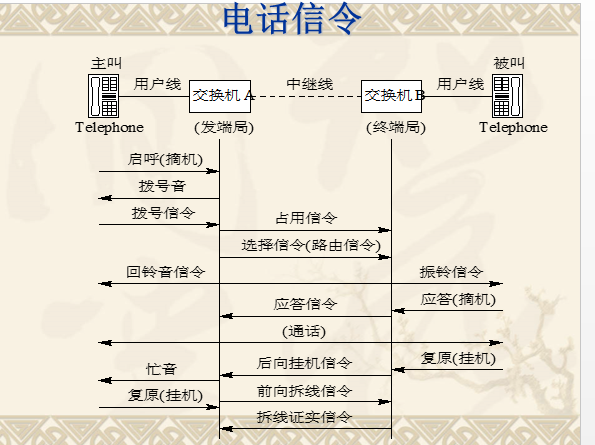
\includegraphics[width=0.7\linewidth]{figures/screenshot024}
			\caption{}
			\label{fig:screenshot024}
		\end{figure}
		\item[计算机通信协议] 采用分层的设计方法。\\
		\textbf{网络的体系结构:}网络的各层功能和协议的集合。\\
		OSI7层模型:上4层为用户层,主要针对用户,下3层为通信层,主要针对通信网。
	\end{description}
\end{enumerate}
\section{对通信网的要求}
\begin{enumerate}
	\item 接通的任意性和快速性
	\item 运行的可靠性
	\item 信息的透明性
	\item 质量的一致性
	\item 较好的灵活性           
	\item 经济的合理性
	
\end{enumerate}
